\documentclass{template/openetcs_report}
% Use the option "nocc" if the document is not licensed under Creative Commons
%\documentclass[nocc]{template/openetcs_article}
\usepackage{lipsum,url}
\graphicspath{{./template/}{.}{./images/}}

\begin{document}
\frontmatter
\project{openETCS}

%Please do not change anything above this line
%============================
% The document metadata is defined below

%assign a report number here
\reportnum{OETCS/WP4/D4.2aV01}

%define your workpackage here
\wp{Work-Package 4: ``Validation \& Verification Strategy''}

%set a title here
\title{openETCS Safety Plan}

%set a subtitle here
\subtitle{Guideline for the safety related activities in an openETCS Onboard Unit development}

%set the date of the report here
\date{October 2013} %\\ Revised March 2013}

%define a list of authors and their affiliation here

\author{Jan Welte}

\affiliation{Technische Universität Braunschweig\\
  Institute for Traffic Safety and Automation Engineering\\
  Langer Kamp 8\\
  38106 Braunschweig, Germany\\
  eMail: openetcs@iva.ing.tu-bs.de \\
  WebSite: www.iva.ing.tu-bs.de}


%add yourself as author, if you contributed to the document



% define the coverart
\coverart[width=350pt]{openETCS_EUPL}

%define the type of report
\reporttype{Output Document}


\begin{abstract}
The safety plan presents an overview about the main safety activities performed during the OpenETCS development process. Thereby, a consistent safety guideline is shown, which combines the functional safety analysis for the system and subsystems from which safety properties will be derived with verification and validation techniques to ensure the overall quality during the design of all safety related parts of the system. Overall, the safety plan will guarantee that the safety design activities required in D2.6 are covered and all safety requirements are fulfilled. 
\end{abstract}

%=============================
%Do not change the next three lines
\maketitle
\tableofcontents
\listoffiguresandtables
\newpage
%=============================

\chapter{Document Control}

\begin{tabular}{|p{4.4cm}|p{8.7cm}|}
\hline
\multicolumn{2}{|c|}{Document information} \\
\hline
Work Package &  WP4  \\
Deliverable ID or doc. ref. & D4.2\\
\hline
Document title & openETCS Safety Plan\\
Document version & 00.01 \\
Document authors (org.)  & Jan Welte (TU-BS)\\
\hline
\end{tabular}

\begin{tabular}{|p{4.4cm}|p{8.7cm}|}
\hline
\multicolumn{2}{|c|}{Review information} \\
\hline
Last version reviewed & -- \\
\hline
Main reviewers & -- \\
\hline
\end{tabular}

\begin{tabular}{|p{2.2cm}|p{4cm}|p{4cm}|p{2cm}|}
\hline
\multicolumn{4}{|c|}{Approbation} \\
\hline
  &  Name & Role & Date   \\
\hline  
Written by    &  Jan Welte & WP4-T4.4 Task Leader  &  October 2013\\
\hline
Approved by & -- & -- & \\
\hline
\end{tabular}

\begin{tabular}{|p{2.2cm}|p{2cm}|p{3cm}|p{5cm}|}
\hline
\multicolumn{4}{|c|}{Document evolution} \\
\hline
00.01 & 01/10/2013 & Jan Welte &  Document creation \\
\hline
Version &  Date & Author(s) & Justification  \\
\hline  
0.10 & 28/01/2014 & Jan Welte &  Extended Introduction  \\
\hline  
\end{tabular}
\newpage

% The actual document starts below this line
%=============================

\mainmatter

\chapter{Introduction}



As the movement characteristics of a train set specific limits in which a driver alone is able to avoid derailment or any kind of collisions railway signaling and protection systems have been developed to ensure safe train movements. Respectively, the mayor parts of a train control system like ETCS include safety relevant functionality. 

\section{Purpose}
\label{sec:purpose}



\section{Document Structure}
\label{sec:document-structure}

This document presents the safety plan, which is closely connected to the V\&V plan, as it presents basic safety activities as well as their specific V\&V activities.

Added by Jan Welte



\section{Safety and Quality}
\label{sec:introduction}



\subsection{Safety}



\subsection{Probabilistic Safety Concept}

\paragraph{Risk}

The EN50128 standard defines safety as the ``freedom from unacceptable levels of risk of harm to people" \cite{EN50128:2011}, which shows that the safety approach required by the CENELEC standards is risk-based. As the risk is defined as the ``combination of the rate of occurrence of accidents and incidents resulting in harm (caused by a hazard) and the degree of severity  of that harm" \cite{EN50128:2011} this approach is based on a probabilistic understanding of event occurrence. The overall relations between all these safety-related terms used to define the safety properties, characteristics and quantities are outlined by the Risk-Genesis-Model of Schnieder, which is shown in the following figure \ref{fig:Risiko-Genese-Modell-eng}.

\begin{figure}[htbp]
\centering
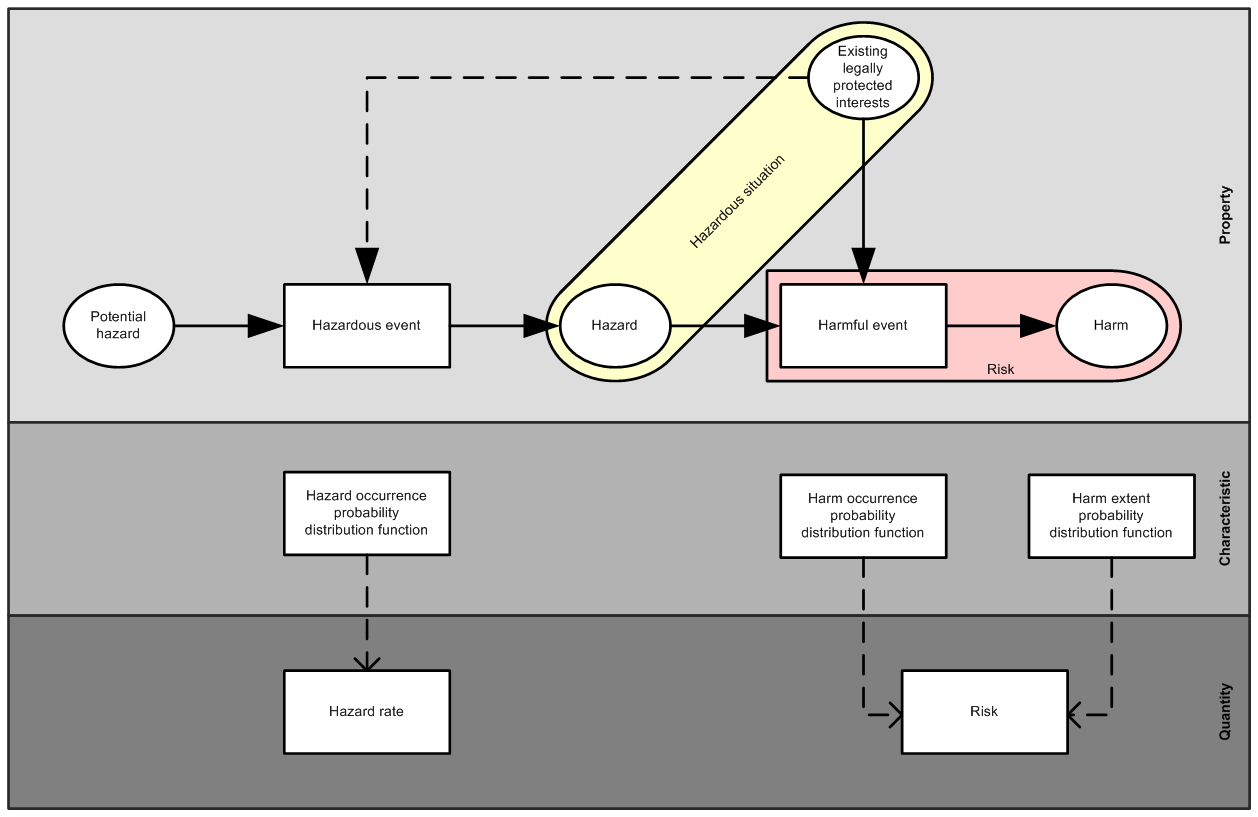
\includegraphics[width=0.7\linewidth]{bld_2013-06-19_Risiko-Genese-Modell-eng-2-0_jw}
\caption{Risk-Genesis-Model showing the relations between the safety-related terms \cite{Schnieder.2010}}
\label{fig:Risiko-Genese-Modell-eng}
\end{figure}

This demonstrates that the first step is to define the system properties, specifically identifying the harms and their related hazardous situations. This has to be performed during a system hazard analysis. Afterwards the respective properties have to be determined by assessing the risk concerning the identified hazards. Based on this work safety integrity levels can be assigned to all system functionalities which are then allocated during the design to certain parts of the operational equipment. As this work is closely related to all design decisions, it has to be done iteratively for all abstraction levels during the system design. 

\begin{figure}[htbp]
\centering
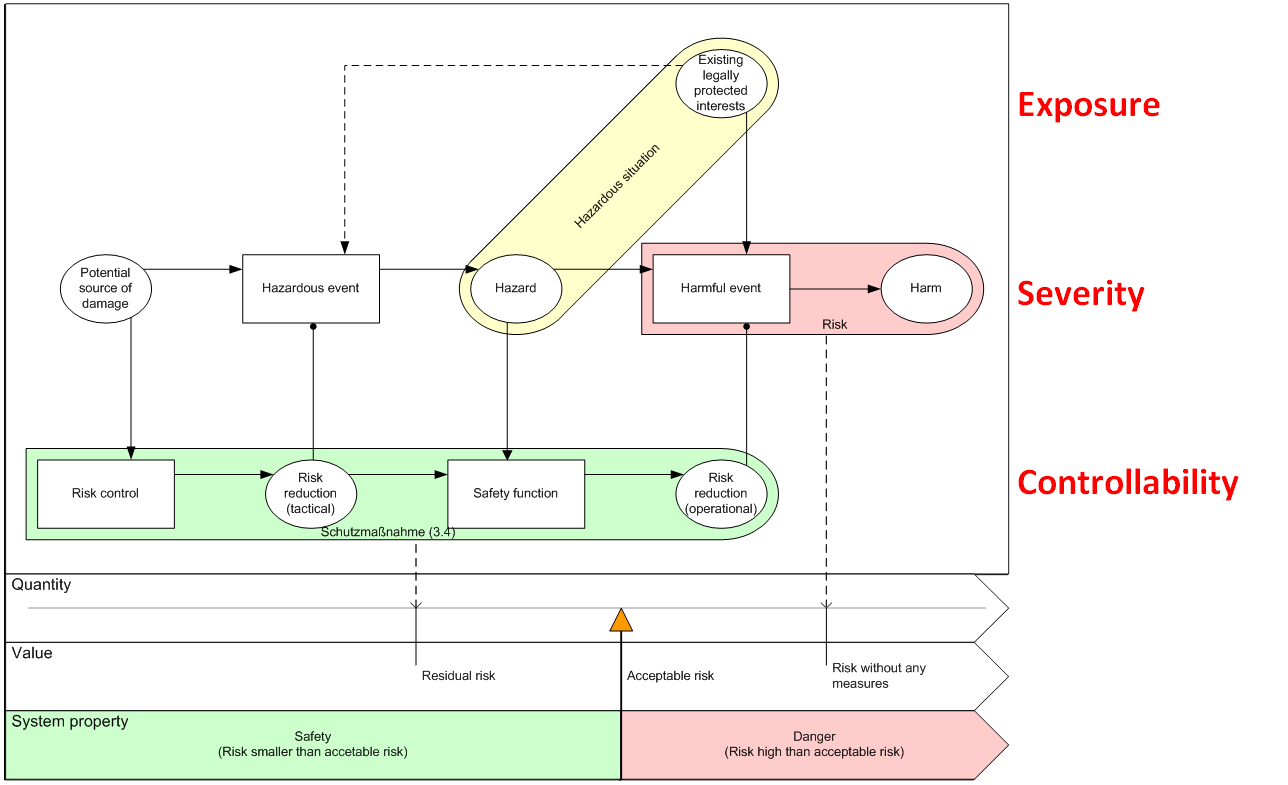
\includegraphics[width=0.7\linewidth]{bld_2013-06-19_Risk-control-modell_1-0_jw}
\caption{Risk control process \cite{Schnieder.2013}}
\label{fig:Risk-control-modell-eng}
\end{figure}

\paragraph{Safety Integrity Level}

The safety integrity level represented the acceptable risk for every part of the system. The risk control process as it is presented in figure \ref{fig:Risk-control-modell-eng} is then performed to ensure that the safety integrity levels are reach by every part of the system.

Since software itself does not fails in the way technical equipment does the specific software safety integrity level represent a qualitative measure with respect to the required degree of correctness for the software functionality than a qualitative value for the likelihood of failing. To reach the needed degree of correctness for the software various design, verification and validation methods are required corresponding to the assigned software safety integrity level. This process leads to safety requirements which have to be implemented in the software design as well as verified and validated. Respectively the EN50126 describes the safety design process as a series of safety tasks for each life cycle phase. This task are related to a number of safety artifacts which are created, used and adapted over time through the different safety design activities.

\textit{Addition topics shall be proposed by every participant.
Section will be managed by Jan Welte}


\subsection{Safety Case}



\subsection{Safety Glossary}

\textbf{Added via the glossary documentation process for openETCS}

\chapter{Document Evolution}

The safety plan will be further specified with the progress of the design process. This specifically reference to the refinement of safety properties on different modeling levels and their corresponding verification and validation methods. All resulting changes and additional safety activities have to be maintained according to the EN~50128.

\begin{description}
\item[V01, T0+16:] First version of the plan. 
\item[V02, T0+17:] First revision, based on the openETCS development process and the preliminary SSRS results. Also the first iteration of V\&V activities will be considered. (D4.2.3)
\item[V03, T0+25:] Second revision, based on the internal reports of modeling and V\&V activities. (D4.3.3)
\item[V04, T0+36:] Final version as part of the final V\&V report (D4.4) 
\end{description}




The first version of the plan is based on the available information of
the design process. This is not yet very detailed as also the
description in Chapter~\ref{cha:vv-design-process} of this report
shows. In particular, the nature of the SSRS is yet to be defined
precisely, and the architecture description including the HW/SW
partitioning needs to be revised.

Concrete plans of activities are thus still to be made, and methods
and tools to be applied will have to be selected. Only the first phase
of V\&V activities is described in Sec.~\ref{sec:first-level-verif}.

\chapter{Safety Strategy}

\textit{This section shall present a short overview about the basic safety aspects apply, the collective strategy for the overall development and who these are applied in the openETCS project.}

\section{Safety Requirements}



\section{Safety Principals}

\textit{This section shall present as short description of all safety principals used for the overall safety strategy.}

\section{Overall Safety Strategy}

\textit{This section shall present as short description for the overall safety strategy.}

\section{OpenETCS Safety Strategy}

\textit{This section shall present the applied openETCS safety strategy.}

\chapter{Safety Process}

\begin{figure}[h]
\centering
\includegraphics[width=0.7\linewidth]{./images/WholeSafetyProcess}
\caption[Overall safety process]{Overall safety process}
\label{fig:SafetyProcess}
\end{figure}

\textit{Process description has to be updated with the latest work. Cooperation between Cyril, Merlin and Jan}

\section{Safety artifacts}

\textit{Process description has to be updated with the latest work. Cooperation between Cyril, Merlin and Jan}

Since all safety design activities are based on the system development activities all system design artifacts are part of the safety design process. Therefore, the following design artifacts of the CENELEC standard development process build the basis for all safety artifacts:

\begin{itemize}
\item System Concept
\item System Requirements Specification
\item Software Requirement Specification
\item Software Architecture Specification
\item Software Design Specification
\item Software Module Design Specification
\item Software Source Code
\end{itemize}

The main safety artifacts are those which are set-up to build the reference for the safety-related aspect during the system development, which are continuously evolved during the design phases. Correspondingly the safety design process has to create artifacts to demonstrated that all safety and quality-related requirements included in the system design. Respectively the following artifacts are created during the safety design process:

\begin{itemize}
\item System Safety Plan
\item Software Quality Assurance Plan
\item Hazard Log
\item System Safety Requirement Specification
\item Safety Case
\end{itemize} 

This artifacts have to be managed over the development process. Since all safety requirement have to be verified and validated there is likewise a close to all Test and Validation Reports.

\section{Safety design activities}
\label{safetyactivities}

\textit{Process description has to be updated with the latest work. Cooperation between Cyril, Merlin and Jan}


The safety design activities set-up or evolve the safety artifacts in relation to the different design artifacts. The following safety design activities are required according to the EN 50128:

\begin{itemize}
\item Preliminary Hazard Analysis
\item Establish Safety Plan
\item System Hazard and Risk Analysis
\item Risk Assessment
\item Specification of System Safety Requirements
\item Define Safety Related Functional Requirements
\item Specify Sub-System and Component Safety requirements
\item Implement Safety Plan
\item Verify System, Sub-System and Component Safety requirements
\item Validate System Safety Requirements
\item Establish Safety Case
\end{itemize}

Overall the safety design activities have to be performed in close relation to the overall verification and validation activities as these have to verify and validate all safety requirements and their results become part of the safety plan.

\section{Safety design process supporting tools}

Supporting software tools are needed to handle the safety artifacts and to some degree to more efficiently perform the safety design activities. As some safety artifacts like the safety requirement specifications and the safety backlogs are closely related to design artifacts the same tools can be used. Especially all requirements should be handled by one tool to ensure full traceability and provide one main interface for the verification and validation activities.

Depending on the methods used for hazard and risk analysis appropriate tools are needed to perform the analysis, collect the hazards and associated risks in the hazard log and to evaluated possible risk control measures. Thereby, traceability has to be guaranteed between all activities.

Since the safety plan and safety case provide the basis for the safety approval the tools used to generated these artifacts should help to generate a consistent argumentation and efficiently collect the data needed to provide evidence. Respectively, interfaces to manage documents and automatically generate reports would be helpful functionalities.

\section{Safety Interfaces}

\textit{Clear description of the interfaces to the process providing inputs for safety and using the Safety results. Specific describing the applied iterations.}

\subsection{Specific Interfaces to the Design Process}

\subsection{Interface to Quality Management}

\subsection{Interface to Verification}

\subsection{Interface to Validation}

\section{Safety Documentation}

\textit{Short description for the needed documentation}

\chapter{OpenETCS Safety Process}

\section{OpenETCS safety design process}

The presented CENELEC standard safety artifacts and activities are always related to the overall system development. Since the openETCS development process just describes the development of the on-board unit software for ETCS additional system informations are needed for the openETCS safety design process. These are mainly the following two parts of the CCS TSI:

\begin{itemize}
\item UNISIG SUBSET-026	System Requirements Specification 	(Version 3.3.0)
\item UNISIG SUBSET-091 Safety Requirements for the Technical Interoperability of ETCS in Levels 1 and 2 	(Version 3.2.0)
\end{itemize}

In relation to SUBSET-91 further documents should be considered:

\begin{itemize}
\item Part of TSI Annex A
	\begin{itemize}
	\item SUBSET-036
	\item SUBSET-037
	\item SUBSET-040
	\item SUBSET-041
	\item SUBSET-098
	\end{itemize}
	
\item Not part of TSI Annex A
	\begin{itemize}
	\item SUBSET-039
	\item SUBSET-078
	\item SUBSET-079
	\item SUBSET-080
	\item SUBSET-081
	\item SUBSET-088
	\end{itemize}
\end{itemize}

From these documents the Preliminary Hazard Analysis and the System Safety Goals have to be derived which are needed as the starting point for the openETCS safety design process. Based on these information a subsystem hazard and risk analysis for the openETCS scope can be performed which set-up the openETCS hazard log. Based on these results the openETCS safety requirements will be specified, which are then further developed to functional requirements. During the development these requirements are adopted if necessary for the different abstraction levels from the high level model down to the source code. This is done using corresponding safety backlogs, which are the reference for the safety requirement verification. Altogether the source code has to be validated against all safety requirements to demonstrated, that software faults can not cause any harm. The safety case has to present all needed documentation.
 
The main task of the openETCS safety design process and the interactions with the design process are shown in figure \ref{fig:WholeSafetyProcess}.

\begin{figure}[htbp]
\centering
\includegraphics[width=0.8\linewidth]{WholeSafetyProcess}
\caption{OpenETCS Safety Design Process}
\label{fig:WholeSafetyProcess}
\end{figure}

The openETCS safety design process will be specified more detailed in the safety plan. Correspondingly, the main safety artifacts and safety design activities which have to be handled during the openETCS safety design process are shown in table \ref{tab:openETCS-Safety-artifacts} and \ref{tab:openETCS-Safety-activities}.

% Table generated by Excel2LaTeX from sheet 'Artifact Categorization'
\begin{table}[htbp]
  \centering
  \caption{Main openETCS safety design process artifacts}
    \begin{tabular}{r|p{8cm}|p{4cm}}
    \textbf{Abbreviation} & \textbf{Safety Artifact} & \textbf{Degree of Formalisation}\\
    \hline
    Safety Req & Safety Requirements: list of all requirements which have to be respected during the system development to reach the safety goals & Informal/ Semi-Formal / Formal \\
    HL    & Hazard Log: List of identified hazards and its associated risk classification as well as information concerning the risk control & Informal \\
    SP    & Safety Plan: Document which specifies all activities, resources and events to ensure that the source code will satisfy all relevant safety requirements & Informal \\
    SC    & Safety Case: Documentation which demonstrates that the used development process and the resulting source code fulfil all safety requirements & Informal \\
    CSB   & Code Safety Backlog: list of requirements/ properties to be implemented inside the dM derived from  the HL (and the dMSB) & Semi-Formal/ Strictly-Formal \\
    dMSB  & Detailed Model Safety Backlog: list of requirements/ properties to be implemented inside the dM derived from the HL (and  the hLSB) & Semi-Formal/ Strictly-Formal \\
    hLSB  & High Level Safety Backlog: list of requirements/ properties to be implemented inside the hM derived from the HL & Informal/ Semi-Formal \\
    \end{tabular}%
  \label{tab:openETCS-Safety-artifacts}%
\end{table}%

\begin{table}[htbp]
  \centering
  \caption{Main openETCS safety design process activities}
    \begin{tabular}{p{4cm}|p{6cm}|p{4cm}} 
 \textbf{Safety Design Activity} & \textbf{Input Artifact(s)} & \textbf{Output Artifact(s)}  \\ \hline
 Establish Safety Plan & QA-Plan + Project documentation (FPP, …) & Safety Plan \\
 Preliminary Hazard Analysis (PHA) & Mainly SUBSET-91(+SUBSET-88) &  Safety Goals + Safety Acceptance Criteria +  PHA report\\ 
 Sub-System Hazard and Risk Analysis (SSHA) & Safety Goals and Acceptance Criteria + SSRS + additional design and architecture specification + additional user constraints  & Hazard Log (incl. Hazards and Safety Functions) \\ 
  Specification of Sub-System Safety Requirements & SUBSET-26 + SUBSET-91 + Hazard Log  & Safety Requirement Specifications \\ 
 Update Hazard Log and corresponding Sub-System Safety Requirements & Verification Reports + Test Cases & Hazard Log + Sub-System Safety Requirements \\
 Specify model specific Requirements & SSRS + Safety Requirement Specification & Safety Plan + Model Backlogs\\
 Verify Safety Requirements & Models + Safety Requirements + Model Backlogs & Verification Report + Verification report \\
 Validate Safety Requirements & Source Code + Safety Requirements & Validation Report + Validation report \\
 Establish Safety Case & V and V Plan + Safety Plan + all requirements and specifications + V and V Reports & Safety Case \\ 
 
\end{tabular}  
  \label{tab:openETCS-Safety-activities}%
\end{table}%

The safety design process and the resulting documentation constitute the main documents for the system approval, as it is required by European and national law to do everything reasonable expectable to prevent harm. Accordingly the CENELEC standards build the common technical rules for the development process. The Common Safety Methods present a concept based on the EN50126 how the risk evaluation and management has to be performed. 

Therefore the main references concerning the safety design process are the CENELEC standards, mainly the EN50126 on how the safety aspects have to be handled as part of the RAMS management over the development process. The overall risk evaluation concept is also defined at this point. The specific concerning the safety case preparations are defined in the EN50129 including the Safety Integrity Level concept. 

Therefore the overall safety management process has to be followed during the openETCS project, as far as it is concerning the scope of openETCS. Therefore the following table \ref{tab:Safety Process Requirements} presents a first list of relevant requirements:

\begin{table}[htbp]
  \centering
  \caption{CENELEC Safety Process Requirements}
    \begin{tabular}{r|r|r}
    Standard & Section & Titel \\
    \hline
     EN 50126 & 4 & Railway RAMS  \\ 
    EN 50126 & 6 & RAMS lifecycle \\
     EN 50128 & Table A.3 & Software Error Effect Analysis\\
    EN 50129 & 5.3 & Evidence of safety management \\
    EN 50129 & Annex A & Safety Integrity Levels \\
    EN 50129 & Annex B & Detailed technical requirements \\
    \end{tabular}%
  \label{tab:Safety Process Requirements}%
\end{table}%

\section{Safety Activities---User Sories}
\label{sec:safety-activ-user}

The VnV Level 1 activities try to implement the overall safety strategy on parts of the benchmark modelling results to establish details for artifact relations, traceability between different artifacts and tool use. Therefore the following benchmark models are used as exemplary design artifacts:

\begin{itemize}
\item SysML model Papyrus by CEA and All4tec

\item Fraunhofer

\item Scade model by Siemens
\end{itemize}

\subsection{Hazardous Events}

Based on the 
\begin{itemize}
\item [a.] KERNEL-6  Manage communication session failure - Related to model of Subset 26 §3.5.3 Establishing a communication session
\item [b.] KERNEL-9  Speed calculation underestimates train speed (or KERNEL-25  Incorrect traction/braking model (Acceleration only)) - Related to model of Subset 26 §3.13 Braking curves
\item [c.] KERNEL-19  Failure of train trip supervision in OS, LS and FS - Related to model of Subset 26 §5.9 Procedure On-Sight
\end{itemize}

\section{Safety Activities View}
\label{sec:safety-activ-proce}
 

\section{OpenETCS Reporting}
\label{sec:safety-reports}

\section{Safety Activities Schedule}
\label{sec:safety-active-time}

\section{Specific Safety Management Procedures}
 
  \textit{This section has to present in close conection with the QA plan how the important procedures, like change management for safety findings or safety evaluation has to be managed.
  
  
  Darstellung der Nachweisführung:
  - Zusammenhang der Argumentationsstruktur
  - Dokumenten Kette
  }
  
\chapter{Conclusion}



\bibliographystyle{unsrt}
\bibliography{erdc}

%===================================================
%Do NOT change anything below this line

\end{document}
